\section{Masinõppe meetodite kvaliteedimõõtude võrdlus}
Uue meetodi kasutusele võtmine tähendab, et on olemas vanem juba kasutuses meetod. Võime kasutada eelnevad meetodit uue hindamiseks. Vana meetodi asendamisel on eelkõige tähtis kas ja kui palju on uus meetod sellest parem. Väljaselgitamiseks uurime meetodite kvaliteedimõõtude vahesid.

Järgnevas laiendame eelmises peatükis sisse toodud tähistusi. Tähistagu $i$-ndat andmepunkti elementide paar $(x_i, y_i)$, kus $x_i$ tähistab andmepunkti tunnuseid ning $y_i$ andmepunkti klassi. Olgu $A$ uus ning $B$ varasem klassifitseerimismeetod, siis saame tähistada andmepunktile vastavaid klassifikatsioone  $A(x_i) = a_i$ ja $B(x_i) = b_i$. Vaadeldes andmepunkti juhusliku suurusena $(X, Y)$ võime meetodite klassifikatsioone sellel vaadelda juhuslike suurustena $A$ ja $B$. Meetodite kvaliteedimõõdud defineerime keskväärtuste kaudu läbi valemite~\eqref{eq:õigsus},~\eqref{eq:täpsus} ja~\eqref{eq:saagis}. Näiteks meetodi $B$ õigsus on $\accuracy_B = \mean{B = Y}$. Eelnevast lähtuvalt saame meetodite erinevuse uurimisel vaadata meetodite kvaliteedimõõtude vahesid
\begin{align}
    \Delta\accuracy &= \mean{A = Y} - \mean{B = Y} \enspace, \label{eq:õigsus vahe} \\
    \Delta\precision &= \mean{A = Y | A = 1} - \mean{B = Y | B = 1} \enspace, \label{eq:täpsus vahe} \\
    \Delta\recall &= \mean{A = Y | Y = 1} - \mean{B = Y | Y = 1} \enspace. \label{eq:saagis vahe}
\end{align}

\subsection{Kvaliteedimõõtude vahede lähendid}
Kuna defineeritud vahede täpseid väärtusi on praktikas keeruline leida hinnatakse neid kasutades valimi keskmisi. Sealjuures on loomulik mõlema meetodi hindamiseks kasutada sama valimit. Ühelt poolt on see standardpraktika - tüüpiliselt hinnatakse masinõppemeetodite edukust fikseeritud testvalimite (\emph{benchmark}) peal. Teisalt tooks kahe valimi kasutamine vajaduse käsitsi märgendada rohkem andmepunkte ning lisab ka lõpptulemusse rohkem juhuslikkust. Kui vastav testvalim sisaldab $N$ andmepunkti, avaldame õigsuste vahe lähendi järgnevalt
\begin{align}
    \Delta \widehat{\accuracy} &= \frac{1}{N} \cdot \sum_{i = 1}^{N} [a_i = y_i] - \frac{1}{N} \cdot \sum_{i = 1}^{N} [b_i = y_i] \nonumber\\
    &= \frac{1}{N} \cdot \sum_{i = 1}^{N} [a_i = y_i] - [b_i = y_i] \nonumber\\
    &= \frac{1}{N} \cdot \sum_{a_i \neq b_i} [a_i = y_i] - [b_i = y_i] \enspace. \label{eq:õigsus vahe lähend}
\end{align}
Saadud võrduses~\eqref{eq:õigsus vahe lähend} on summa märgi all nullist erinev arv parajasti siis, kui meetodite klassifikatsioonid on erinevad. Sellest järeldub, et meetodite õigsuste vahe hindamiseks peame märgendama vaid andmepunkte, kus $a_i \neq b_i$. Näiteks kui meetodid on õigsustega üle $90\%$ võivad nende klassifikatsioonid erineda maksimaalselt $20\%$ andmetest. Sellisel juhul peaksime märgendama vaid iga viienda andmepunkti. Veelgi enam, kuna iga summa liige valemis~\eqref{eq:õigsus vahe lähend} on $\pm 1$, on võimalik hinnata $\Delta \widehat{\accuracy}$ ilma ühtegi andmepunkti märgendamata
\begin{equation}
    \label{eq:õigsus vahe lähend tõke}
    | \Delta \widehat{\accuracy} | \leq \frac{\# \{i: a_i \neq b_i \}}{N} \enspace,
\end{equation}
kus murru lugejas tähistab $\#$ hulga suurust. Seega saame veenduda, kas kaks algoritmi üldse õigsuse poolest erinevad andmepunktide tegelikke klasse teadmata.

Analoogselt õigsusele avaldame ka valimipõhiste täpsushinnangute vahe
\begin{equation}
    \label{eq:täpsus vahe lähend kole}
    \Delta \widehat{\precision} = \frac{\sum \limits_{i = 1}^{N} [a_i = 1] \cdot [y_i = 1]}{\sum \limits_{i = 1}^N [a_i = 1]} - 
    \frac{\sum \limits_{i = 1}^{N} [b_i = 1] \cdot [y_i = 1]}{\sum \limits_{i = 1}^N [b_i = 1]} \enspace,
\end{equation}
mille edasise lihtsustamise teeb raskeks erinevus murru nimetajates. Kuna tehniliselt ei pea täpsuse hindamisel kasutama sama testvalimit mõlema algoritmi jaoks, võime esialgset testvalmit kitsendada nii, et murru lugejad langevad kokku
\begin{equation*}
    \sum_{i = 1}^{N_A} [a_i = 1] = S = \sum_{i = 1}^{N_B} [b_i = 1] \enspace,
\end{equation*}
ning $N = \max (N_A, N_B)$.
Selline lähenemine on samaväärne valikumeetodi põhjal kahe $S$ andmepunktise valimi moodustamisega, kus vastuvõtutingimused on vastavalt $a_i = 1$ ja $b_i = 1$. Seda arvestades saame valemi~\eqref{eq:täpsus vahe lähend kole} viia lihtsustatud kujule
\begin{equation*}
     \Delta \widehat{\precision} = \frac{1}{S} \cdot \sum_{i = 1}^{N_A} [a_i = 1] \cdot [y_i = 1] - \frac{1}{S} \cdot \sum_{i = 1}^{N_B} [b_i = 1] \cdot [y_i = 1] \enspace,
\end{equation*}
kus $a_i$ on määratud vaid esimesel $N_A$ ja $b_i$ on määratud vaid esimesel $N_B$ andmepunktil. Seega on $a_i$ ja $b_i$ väärtus kõigi $N$ punkti seas kas määramata, $0$ või $1$. Siit lähtuvalt
\begin{align}
    \Delta \widehat{\precision} &= \frac{1}{S} \cdot \left( \sum_{\substack{a_i = 1 \\ b_i = 1}} [y_i = 1] + \sum_{\substack{a_i = 1 \\ b_i \neq 1}} [y_i = 1] - \sum_{\substack{a_i = 1 \\ b_i = 1}} [y_i = 1] - \sum_{\substack{a_i \neq 1 \\ b_i = 1}} [y_i = 1] \right) \nonumber\\
    &= \frac{1}{S} \cdot \left( \sum_{\substack{a_i = 1 \\ b_i \neq 1}} [y_i = 1] - \sum_{\substack{a_i \neq 1 \\ b_i = 1}}[y_i = 1] \right) \nonumber\\
    &= \frac{1}{S} \cdot \sum_{a_i \neq b_i} [a_i = 1] \cdot [y_i = 1] - [b_i = 1] \cdot [y_i = 1] \enspace. \label{eq:täpsus vahe lähend}
\end{align}
Andmepunktide märgendamise mõttes on täpsuse vahe lähend~\eqref{eq:täpsus vahe lähend} samaväärne õigsuse valemiga~\eqref{eq:õigsus vahe lähend}, sest hinnangu arvutamiseks peame märgendama vaid andmepunkte, mille puhul $a_i\neq b_i$.

Täpsuse vahehinnangu praktiline arvutamine algab $S$ fikseerimisest. Seejärel rakendame valimile meetodeid kuni kumbki on $S$ andmepunkti positiivseks klassifitseerinud. Märgendama peame valimi andmepunktid, mille puhul on olemas mõlema meetodi klassifikatsioonid ning mis on üksteisest erinevad. Nüüd saame arvuta summa liikmete väärtused ning seejärel hinnangu täpsuste vahele. Sellega oleme oluliselt vähendatud märgendamist vajavate andmete hulka.

Saagise vahe avaldame sarnaselt täpsusele, lähtudes valemist
\begin{equation*}
    \Delta \widehat{\recall} = \frac{\sum \limits_{i = 1}^{N} [a_i = 1] \cdot [y_i = 1]}{\sum \limits_{i = 1}^{N} [y_i = 1]} - \frac{\sum \limits_{i = 1}^{N} [b_i = 1] \cdot [y_i = 1]}{\sum \limits_{i = 1}^{N} [y_i = 1]} \enspace,
\end{equation*}
kus erinevalt täpsusest on murdude nimetajad definitsiooni järgi võrdsed. Tähistagu nimetajas olevat summat
\begin{equation*}
    T = \sum_{i = 1}^N [y_i = 1] \enspace.
\end{equation*}
Korrates täpsuse valemi~\eqref{eq:täpsus vahe lähend} tuletamisega analoogset mõttekäiku, võime esitada saagise vahe hinnangu kujul
\begin{equation}
    \label{eq:saagis vahe lähend}
    \Delta \widehat{\recall} = \frac{1}{T} \cdot \sum_{a_i \neq b_i} [a_i = 1] \cdot [y_i = 1] - [b_i = 1] \cdot [y_i = 1] \enspace. 
\end{equation}
Märgendamise seisukohalt on $T$ arvutamine kulukas, kuna iga summa liikme puhul on vajalik teada andmepunkti tegelikku klassi. Kõigi $N$ andmepunkti manuaalne märgendamine on väga ressursimahukas. Alternatiivina saame väiksema valimi põhjal positiivse klassi esinemise sagedust ennustada. See on võimalik vaid siis kui positiivse klassi esinemise sagedus on piisavalt suur. Kui positiivse klassi esindajad on sagedusega $1:1000$, peaksime adekvaatse hinnangu saamiseks läbi vaadama üle kümnetuhande andmepunkti. Seega on valemi~\eqref{eq:saagis vahe lähend} praktiline rakendamine raskendatud veelgi madalama esinemissagedusega sündmuste korral.

\subsection{Õigsuste vahe lähendamine}
Siiani oleme lähendeid kvaliteedimõõtude vahele avaldatud vahetult läbi vahe oodatud väärtuse definitsiooni. Tehes teisendusi vahe definitsioonis antud avaldises võime selle eraldada mitmeks komponendiks. Lõpliku lähendi leidmiseks peame lähendama iga komponenti eraldi ning nende põhjal arvutama vahele hinnangu.

Olgu meil kaks klassifitseerimismeetodit koos juhusliku andmepunkti $Y$ klassifitseerimisele vastavate juhuslike suurustega $A$ ja $B$. Siis saame valemi~\eqref{eq:õigsus vahe} kirjutada lahti vastavalt definitsioonile
\begin{equation}
    \label{eq:õigus vahe definitsiooni järgi keskväärtuste kaudu}
    \Delta \accuracy = \mean{A = Y} - \mean{B = Y} = \mean{[A = Y] - [B = Y]} \enspace.
\end{equation}
Tähistagu $Z$ valemis~\eqref{eq:õigus vahe definitsiooni järgi keskväärtuste kaudu} viimase keskväärtusmärgi all olevat juhuslikkus suurust, $Z = [A = Y] - [B = Y]$. Analoogselt võime valemis~\eqref{eq:õigsus vahe lähend} oleva summa liikmeid tõlgendada juhuslike suurustena $Z_i = [a_i = y_i] - [b_i = y_i]$. Kui arvestame, et juhuslikud suurused $Z_i$ on sõltumatud ning sama jaotusega kui $Z$, näeme et lähendi~\eqref{eq:õigsus vahe lähend} keskväärtus on
\begin{equation}
    \mean{\Delta \widehat{\accuracy}} = \frac{1}{N} \cdot \sum_{i = 1}^N \cdot \mean{Z_i} = \Delta \accuracy \enspace.
\end{equation}
See tähendab, et $\widehat{\accuracy}$ on nihketa hinnang õigsuste vahele. Kuna meetodite erinevus avaldub sündmustes, kus meetodite klassifikatsioonid erinevad ($Z \neq 0$), võime $\Delta \accuracy$ avaldada just selliste sündmuste kaudu
\begin{align*}
    \Delta \accuracy &= \prob{Z = 0} \cdot \mean{Z \mid Z = 0} + \prob{Z \neq 0} \cdot \mean{Z \mid Z \neq 0} \\
    &= \prob{Z \neq 0} \cdot \mean{Z \mid Z \neq 0} \enspace.
\end{align*}
Edasiste arvutuste selgemaks esitamiseks võtame kasutusele tähistused
\begin{align}
    \beta &= \prob{Z \neq 0} \enspace, \label{eq:beta} \\
    \gamma &= \mean{Z | Z \neq 0} \enspace, \label{eq:gamma} \\
    \kappa &= \prob{Z = 1 | Z \neq 0} \enspace. \label{eq:kappa}
\end{align}
Need kolm suurust pole sõltumatud parameetrid. Keskväärtuse definitsioonist lähtuvalt on $\gamma$ ja $\kappa$ omavahel seotud
\begin{equation*}
    \gamma = \mean{Z | Z \neq 0} = 1 \cdot \kappa - 1 \cdot (1 - \kappa) = 2 \kappa - 1 \enspace,
\end{equation*}
ning me saame esitada õigsuste vahe antud suuruste kaudu
\begin{equation}
    \label{eq:õigsus vahe tähistega}
    \Delta \accuracy = \beta \cdot \gamma = \beta \cdot (2 \kappa - 1) \enspace.
\end{equation}

Võrdusest~\eqref{eq:õigsus vahe tähistega} lähtuvalt hindame meetodite õigsuste vahet lähendades suurusi $\beta$ ja $\gamma$. Kuna $\beta = \prob{Z \neq 0}$ on tõenäosus, saame seda hinnata statistilise tõenäosusena üle $N$ elemendilise valimi 
\begin{equation}
    \label{eq:beta lähend}
    \hat{\beta} = \frac{1}{N} \cdot \sum_{i = 1}^{N} [Z_i \neq 0] = \frac{1}{N} \cdot \sum_{i = 1}^{N} [a_i \neq b_i] \enspace,
\end{equation}~\cite{rakendusstatisika-algkursus}.
Summa märgi alune juhuslik suurus võtab väärtusi $0$ ja $1$. See tähendab, et lähendi absoluutse ja relatiivse vea hinnangud saame leida eelmises peatükis kirjeldatud meetodeid kasutades.

Lähendi tinglikule keskväärtusele $\gamma = \mean{Z \mid Z \neq 0}$ on leiame sarnaselt, valimikeskimisena kus iga valimi andmepunkti korral $a_i \neq b_i$. Olgu $K$ sellise valimi suurus, esitame lähendi kujul
\begin{equation}
    \label{eq:gamma lähend}
    \hat{\gamma} = \frac{1}{K} \cdot \sum_{i = 1}^K [a_i = y_i] - [b_i = y_i] \enspace.
\end{equation}
Kuna lähendis $\hat{\gamma}$ on summa liikmete võimalikud väärtused $-1$ ja $1$, ei ole summa liikmed Bernoulli jaotusega. See-eest on ikka tegu binaarse tunnusega, mille põhjal defineerime uue Bernoulli jaotusega juhusliku suuruse $W$, mis võtab väärtuse $0$ kui summeritav suurus võtab $-1$ ning muidu $1$
\begin{equation*}
    W = \frac{Z + 1}{2} \enspace,
\end{equation*}
mille puhul
\begin{align*}
    \prob{W = 1} &= \prob{Z = 1 | Z \neq 0} = \kappa \enspace, \\
    \prob{W = 0} &= \prob{Z = -1 | Z \neq 0} = 1 - \kappa \enspace.
\end{align*}
Sündmusena on uus defineeritud suurus samaväärne vanaga, endiselt võime rakendada binoomjaotusel põhinevaid tulemusi eelmisest peatükist. Lähtume võrrandist
\begin{equation*}
    \prob{\left| \frac{\hat{\gamma}}{\gamma} - 1 \right| \geq \varepsilon} = \alpha \enspace,
\end{equation*}
ning kordama sama mõttekäiku, mis valemi~\eqref{eq:binoomjaotus relatiivne viga} puhul.

Leitud lähendite korrutisest leiame omakorda lähendi meetodite õigsuste vahele
\begin{equation*}
    \Delta \widehat{\accuracy} = \hat{\beta} \cdot \hat{\gamma} \enspace.
\end{equation*}
Vahe lähendi relatiivse vea dispersioon avaldame relatiivse vea korrutise omaduse~\eqref{eq:korrutise relatiivne viga dispersioon ligikaudne} põhjal
\begin{equation}
    \variance{\frac{\hat{\beta} \cdot \hat{\gamma}}{\beta \cdot \gamma}} \approx \variance{\frac{\hat{\beta}}{\beta}} + \variance{\frac{\hat{\gamma}}{\gamma}} \enspace,
\end{equation}
kus hinnangute $\hat{\beta}$ ja $\hat{\gamma}$ relatiivsete vigade dispersioonid on
\begin{align}
    \variance{\frac{\hat{\beta}}{\beta}} &= \frac{1}{N} \cdot \frac{1 - \beta}{\beta} \enspace, \label{eq:beta relatiivne viga dispersioon} \\
    \variance{\frac{\hat{\gamma}}{\gamma}} &= \frac{1}{K} \cdot (\mean{Z^2 | Z \neq 0} - \mean{Z | Z\neq 0}^2) = \frac{1}{K} \cdot (1 - \gamma^2) \enspace. \label{eq:gamma relatiivne viga dispersioon}
\end{align}
\begin{figure}[H]
    \begin{center}
        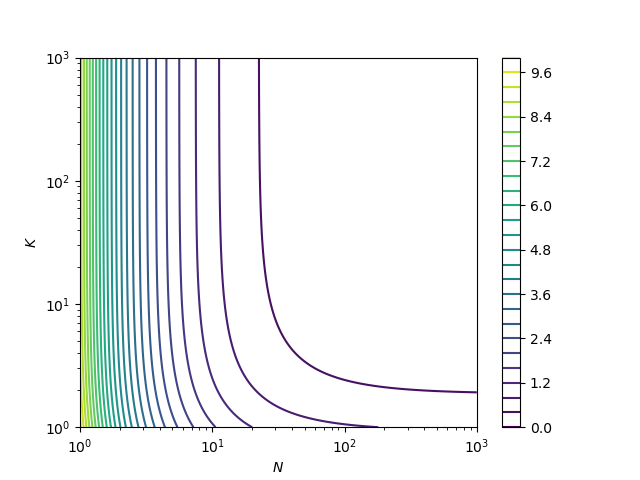
\includegraphics[width=\textwidth]{oigsus_vahe_relatiive_viga_dispersioon}  
    \end{center}
    \caption{Õigsuste vahe lähendi relatiivse vea dispersioon juhusliku valimi suuruse $N$ ning märgendatud tingliku $(a_i \neq b_i)$ valimi suuruse $K$ suhtes. Juhul kui $\Delta \accuracy = 5\%$ ja $\beta = 10\%$. Heledus tähistab dispersiooni.}
    \label{fig:õigsus vahe lähend relatiivne viga dispersioon}
\end{figure}

Joonise~\ref{fig:õigsus vahe lähend relatiivne viga dispersioon} ning vahetulemuste~\eqref{eq:beta relatiivne viga dispersioon} ja~\eqref{eq:gamma relatiivne viga dispersioon} kaudu näeme, et $\Delta \widehat{\accuracy}$ relatiivse vea dispersioon kahaneb valimisuuruste kasvades. Telgedel olevatest suurustest tähistab $N$ valimi suurust, mida ei pea märgendama. Kuna sellise valimi leidmine ei ole keeruline võime eeldada, et $N$ on fikseeritud ja küllaltki suur. Oluline on aga suurus $K$, mis tähistab märgendamist vajavate andmepunktide arvu. Märgendatud valimi suuruse prognoosimiseks fikseeritud $N$ põhjal uurime olukorda, kus saavutame võrdsed lähendite $\hat{\beta}$ ja $\hat{\gamma}$ dispersioonid
\begin{equation}
    \label{eq:võrdsed vahe relatiivse vea dispersioonid}
    \frac{1}{N} \cdot \frac{1 - \beta}{\beta} = \frac{1}{K} \cdot (1 - \gamma^2) \enspace.
\end{equation}
Kuna $\Delta \accuracy = \beta \cdot \gamma$, saame valemi~\eqref{eq:võrdsed vahe relatiivse vea dispersioonid} esitata kujul
\begin{equation}    
    K = N \cdot \frac{\beta}{1-\beta} \cdot \left( 1 - \frac{(\Delta\accuracy)^2}{\beta^2} \right) \enspace,
\end{equation}
mille põhjal saame hinnata märgendamist vajava valimi suurust.

\subsection{Saagiste vahe lähendamine}
Saagise puhul on hinnangu~\eqref{eq:saagis vahe lähend} analüüsimine keerulisem, kuna saagise definitsioonis on tinglik keskväärtus. Valemile~\eqref{eq:õigsus vahe tähistega} analoogi tuletamiseks peame kõigepealt eraldama saagise definitsioonist tingliku jaotuse
\begin{align*}
    \mean{A = Y | Y = 1} &= \mean{A = 1 | Y = 1} = \prob{A = 1 | Y = 1} \enspace, \\
    \mean{B = Y | Y = 1} &= \mean{B = 1 | Y = 1} = \prob{B = 1 | Y = 1} \enspace,
\end{align*}
millest saame tuletada
\begin{equation*}
    \mean{A = Y | Y = 1} =\frac{\prob{A = 1 \land Y = 1}}{\prob{Y = 1}} = \frac{\mean{[A = 1] \cdot [Y = 1]}}{\mean{Y = 1}} \enspace.
\end{equation*}
Analoogselt meetodi $B$ puhul
\begin{equation*}
    \mean{A = Y | Y = 1} = \frac{\prob{B = 1 \land Y = 1}}{\prob{Y = 1}} = \frac{\mean{[B = 1] \cdot [Y = 1]}}{\mean{Y = 1}} \enspace.
\end{equation*}
Nende kahe võrduse põhjal esitame saagiste vahe kujul
\begin{align*}
    \Delta \recall &= \mean{A = Y | Y = 1} - \mean{B = Y | Y = 1} \\
    &= \frac{\mean{[A = 1] \cdot [Y = 1] - [B = 1] \cdot [Y = 1]}}{\mean{Y = 1}} \enspace.
\end{align*}
Sellest saame järeldada algse saagise lähendi valemi~\eqref{eq:saagis lähend} põhjal, et ka saagiste vahe lähend~\eqref{eq:saagis vahe lähend} on nihketa. Kuid sellisel kujul esitatud vahele $\Delta \recall$ ei ole lähendi leidmine märgendamise seisukohalt veel kõige parem.

Kehtivad seosed
\begin{align*}
    \mean{[A = 1] [Y = 1]} &= \mean{[A = 1] [Y = 1] [B = 1]} + \mean{[A = 1] [Y = 1] [B = 0]} \enspace, \\
    \mean{[B = 1] [Y = 1]} &= \mean{[B = 1] [Y = 1] [A = 1]} + \mean{[B = 1] [Y = 1] [A = 0]} \enspace,
\end{align*}
nende seoste ja keskväärtuse definitsiooni põhjal esitame saagise vahe lugeja korrutisena tõenäosusest ja tinglikust keskväärtusest
\begin{align*}
    &\mean{[A = 1] [Y = 1] - [B = 1] [Y = 1]} \\
    &= \mean{[A = 1] [Y = 1] [A \neq B] - [B = 1] [Y = 1] [A \neq B]} \\
    &= \prob{A \neq B} \cdot \mean{[A = 1] [Y = 1] - [B = 1] [Y = 1] | [A \neq B]} \enspace.
\end{align*}
Edasiste arvutuste selgemaks esitamiseks võtame jällegi kasutusele abistavad tähistused
\begin{align*}
    \beta &= \prob{A \neq B} \enspace, \\
    \nu &= \prob{Y = 1} \enspace, \\
    \eta &= \mean{[A = 1] [Y = 1] - [B = 1] [Y = 1] | [A \neq B]} \enspace,
\end{align*}
mille kaudu saame esitada saagiste vahe
\begin{equation}
    \label{eq:saagis vahe tähistega}
    \Delta \recall = \frac{\beta \cdot \eta}{\nu} \enspace.
\end{equation}

Tulemuse~\eqref{eq:saagis vahe tähistega} põhjal on võimalik meetodite saagiste vahet hinnata kui lähendame suurusi $\beta$, $\nu$ ja $\eta$. Tõenäosuse $\beta$ puhul saame hinnang leida samamoodi nagu~\eqref{eq:beta lähend} eelmises alampeatükis. Ning $\nu$ lähendi sarnaselt üle $N$ suuruse juhusliku valimi
\begin{align*}
    \hat{\beta} &= \sum_{i = 1}^N [a_i \neq b_i] \enspace, \\
    \hat{\nu} &= \sum_{i = 1}^N [y_i = 1] \enspace.
\end{align*}
Tinglikku keskväärtust $\eta$ lähendame valimikeskmisena üle tingliku valimi, kus $a_i \neq b_i$. Olgu selle valimi suurus $K$, siis
\begin{equation*}
    \hat{\eta} = \frac{1}{K} \cdot \sum_{i = 1}^K [a_i = 1] [y_i = 1] - [b_i = 1] [y_i = 1] \enspace.
\end{equation*}
Kuna hinnangute $\hat{\beta}$ ja $\hat{\nu}$ puhul on summa liikmete võimalikud väärtused $0$ ja $1$, on lähendite absoluutse ja relatiivse vea hinnangud leitavad meetoditega eelmisest peatükist. Kuna lähendi $\hat{\eta}$ puhul on summa liikmete võimalikud väärtused $-1$, $0$, ja $1$, ei saa rakendada binoomjaotusel põhinevaid tulemusi. See-eest saame endiselt kasutada Höffdinig võrratust lähendi absoluutse vea hindamiseks, seekord tõketega $-1$ ja $1$, mille põhjal avaldub valimi vajalik suurus
\begin{equation*}
    K \geq - \frac{2}{\varepsilon^2} \cdot \ln{\left( \frac{\alpha}{2} \right)} \enspace,
\end{equation*}
kus $\varepsilon$ on absoluutse vea absoluutväärtuse maksimaalset lubatud suurust ning $\alpha$ olulisus.

Relatiivse vea korrutise~\eqref{eq:korrutise relatiivne viga dispersioon ligikaudne} ja jagatise~\eqref{eq:jagatis relatiivne viga dispersioon} dispersiooni omaduste põhjal esitame saagise vahe hinnangu relatiivse vea dispersiooni summana
\begin{equation*}
    \variance{\frac{\hat{\beta} \cdot \hat{\eta}}{\hat{\nu}} \div \frac{\beta \cdot \eta}{\nu}} \approx \variance{\frac{\hat{\beta}}{\beta}} + \variance{\frac{\hat{\nu}}{\nu}} + \variance{\frac{\hat{\eta}}{\eta}} \enspace,
\end{equation*}
millest
\begin{equation*}
    \variance{\frac{\hat{\beta}}{\beta}} = \frac{1}{N} \cdot \frac{1 - \beta}{\beta}, \qquad \variance{\frac{\hat{\nu}}{\nu}} = \frac{1}{N} \cdot \frac{1 - \nu}{\nu} \enspace. \\
\end{equation*}

\subsection{Täpsuste vahe lähendamine}
Täpsuse jaoks on võrrandi~\eqref{eq:saagis vahe tähistega} analoogi tuletamine keeruline, sest täpsuste vahe lähendis on summa liikmed mittesõltumatud. Üheks võimalikuks lahenduseks täpsuse hindamisel on kahesammuline lähenemine, kus hindame esmalt lähendi~\eqref{eq:täpsus vahe lähend kole} dispersiooni funktsioonina valikumeetodi abil saadud $S$ elemendilisest valimist (kahe keskmise vahe) ning seejärel lähendame selle optimeeritud esitust~\eqref{eq:täpsus vahe lähend} veelgi väiksema $K$-elemendilise juhuvalimiga. Kuna saadud lahendus ei ole elegantne ning kõik sammud iseseisvalt on analoogsed peatükis~\ref{section:kvaliteedimõõtude veahinnangud} saadud tulemustega, siis ei me seda antud töös pikemalt ei käsitle.